
\documentclass[conference]{IEEEtran}
\IEEEoverridecommandlockouts
% The preceding line is only needed to identify funding in the first footnote. If that is unneeded, please comment it out.
\usepackage{cite}
\usepackage{amsmath,amssymb,amsfonts}
\usepackage{algorithmic}
\usepackage{graphicx} 
\usepackage{array}   
\usepackage{multirow} 
\usepackage{textcomp}
\usepackage{amsmath}
\usepackage{xcolor}
\usepackage{blindtext}
\usepackage{hyperref}
\usepackage{multirow}
\usepackage{float}
\usepackage{stfloats}
\usepackage{longtable}
\usepackage{booktabs}
\usepackage{pdflscape} % For landscape pages
% \usepackage{caption}
\raggedbottom


% --- Begin Arabic Support Additions ---
\usepackage[english]{babel}
\usepackage{arabtex}
\usepackage{utf8}
\setcode{utf8}     
% --- End Arabic Support Additions ---

\usepackage [autostyle, english = american]{csquotes}
\MakeOuterQuote{"}

% Define a custom command for formatting Arabic text
\newcommand{\artext}[1]{%
  {\fontsize{8pt}{11pt}\selectfont \raisebox{0pt}[0pt][0pt]{\RL{#1}}}%
}


\def\BibTeX{{\rm B\kern-.05em{\sc i\kern-.025em b}\kern-.08em
    T\kern-.1667em\lower.7ex\hbox{E}\kern-.125emX}}

\makeatletter
\newcommand{\linebreakand}{%
  \end{@IEEEauthorhalign}
  \hfill\mbox{}\par
  \mbox{}\hfill\begin{@IEEEauthorhalign}
}





\begin{document}

\title{From Script to Digital: A Deep Learning Approach to Arabic Handwriting Recognition}

\author{
    \IEEEauthorblockN{Hamza Ahmed Abushahla\textsuperscript{*}}
    \IEEEauthorblockA{\textit{Department of Computer Science and Engineering} \\
    \textit{American University of Sharjah}\\
    Sharjah, United Arab Emirates \\
    b00090279@aus.edu}
    %
    \and
    %
    \IEEEauthorblockN{Ariel Justine Navarro Panopio\textsuperscript{*}}
    \IEEEauthorblockA{\textit{Department of Computer Science and Engineering} \\
    \textit{American University of Sharjah}\\
    Sharjah, United Arab Emirates \\
    b00088568@aus.edu}
    %
    \linebreakand
    %
    \IEEEauthorblockN{Layth Al-Khairulla\textsuperscript{*}}
    \IEEEauthorblockA{\textit{Department of Computer Science and Engineering} \\
    \textit{American University of Sharjah}\\
    Sharjah, United Arab Emirates \\
    b00087225@aus.edu} %test
    %
    \and
    %
    \IEEEauthorblockN{Alex Aklson\textsuperscript{†}}
    \IEEEauthorblockA{\textit{Department of Computer Science and Engineering} \\
    \textit{American University of Sharjah}\\
    Sharjah, United Arab Emirates \\
    aaklson@aus.edu}
    %
    \thanks{\textsuperscript{*}These authors contributed equally to this work.}
        \thanks{\textsuperscript{†}Author to whom correspondence should be addressed.}
}

\maketitle

\begin{abstract}
Handwritten Text Recognition (HTR) for Arabic script is crucial for enabling digital accessibility and automating the conversion of handwritten documents into searchable digital formats. The cursive nature of Arabic script, with its positional letter shapes and diacritical marks, presents significant challenges that require specialized recognition systems. These challenges are compounded by the variability in handwriting styles and the limitations of techniques developed for other languages.
In this study, we leverage the KHATT dataset to develop an end-to-end deep learning-based HTR system. Our approach effectively addresses the complexities of Arabic cursive handwriting using a segmentation-based model. This work demonstrates the potential of deep learning in advancing Arabic HTR, enabling the digitization of both contemporary and historical texts and supporting broader applications in cultural preservation and digital workflows.
\end{abstract}

% \vspace{-10pt}

\begin{IEEEkeywords}
Arabic Handwriting Recognition, KHATT Dataset, Arabic Handwriting, Optical Character Recognition, Deep Learning, Cursive Text Recognition
\end{IEEEkeywords}

\section{Introduction}

The Arabic language is the official language of 24 sovereign countries and is spoken by over 400 million people worldwide \cite{saeed2024muharaf}. It is also one of the six official working languages of the United Nations (UN), reflecting its international importance. Beyond its widespread use, Arabic holds profound cultural, literary, and religious significance, serving as a cornerstone of the heritage of Arab and Muslim communities globally \cite{ayuba2013}. This extensive reach emphasizes the importance of developing accurate Arabic handwritten text recognition (HTR) systems, which have diverse applications in educational, governmental, and cultural preservation contexts \cite{mutawa2024machine}. For instance, the ability to accurately convert both historical and contemporary handwritten Arabic documents into digital text is vital for the digitization of archives, streamlining administrative processes, and supporting large-scale data analysis efforts.

\begin{figure}[t]
  \centering
  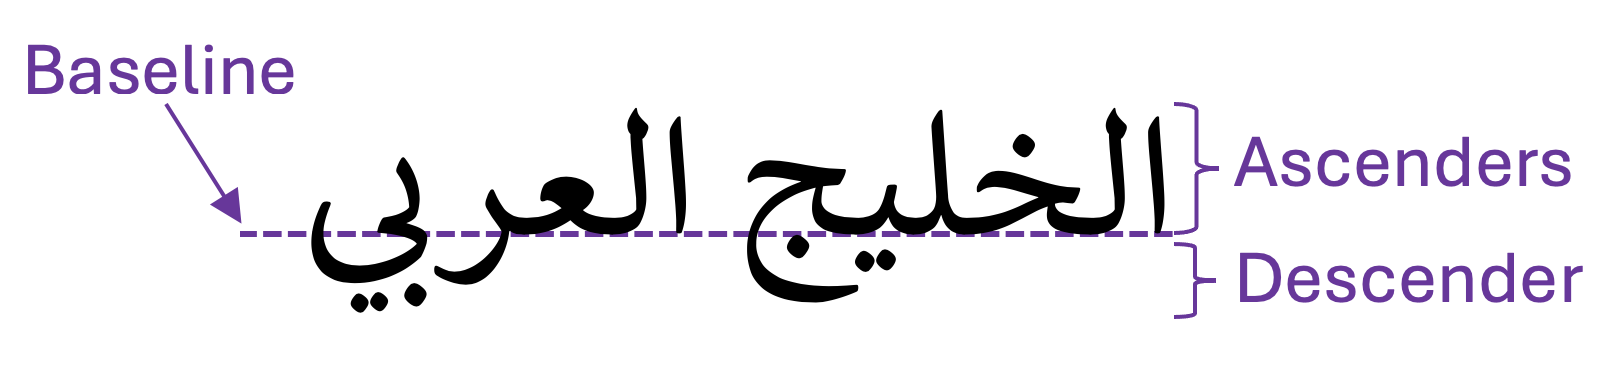
\includegraphics[width=0.9\linewidth]{Figs/fig2.png}
  \caption{Sample line images from the KHATT dataset \cite{mahmoud2014khatt}.}
  \label{fig:engagement_examples}
\end{figure}



In particular, the automated recognition and digitization of Arabic cursive handwriting present unique challenges due to the inherent complexities of the script. For one, Arabic is written from right to left, with letters assuming different shapes based on their positional context within words. In addition, diacritical marks, known as "\artext{حركات}" (harakat), and other special symbols such as the "\artext{همزة}" (hamza) and "\artext{مدّة}" (madda) further complicate the digitization process, as many letters share identical base shapes but are distinguished by one or more dots placed above or below the character \cite{el1990arabic}. These characteristics, combined with the variability in individual handwriting styles, make the task of accurately recognizing and digitizing Arabic handwriting particularly demanding. Furthermore, because of these unique challenges, techniques developed for recognizing handwriting in other languages, such as Latin-based scripts, cannot be directly applied to Arabic, necessitating tailored approaches and specialized models \cite{alrobah2022arabic}.

Traditional Arabic HTR systems have predominantly relied on shallow learning techniques \cite{mutawa2024machine}. These methods typically involve handcrafted feature extraction processes that are sensitive to noise and degradation, limiting their effectiveness and scalability \cite{parvez2013offline}. Furthermore, most existing systems adopt a segmentation-based approach, requiring the segmentation of words into individual characters before recognition. This segmentation process is particularly challenging for Arabic due to the cursive connections between letters and the presence of similar character shapes, making it difficult to accurately isolate each character \cite{faizullah2023survey, mezghani2023recent}. In contrast, segmentation-free models (holistic approaches) recognize words as whole-word images without any segmentation processes, which can be more effective for specific applications with limited vocabularies \cite{alkhateeb2009component, nashwan2017holistic}.

Over the past decade, significant advancements in deep learning have revolutionized the field of HTR. Convolutional Neural Networks (CNNs) have emerged as the foundation of modern HTR systems due to their ability to extract complex spatial features, making them particularly effective for cursive scripts like Arabic \cite{mosbah2024adocrnet, alrobah2022arabic, altwaijry2021arabic}. Combined with Bidirectional Long Short-Term Memory (BiLSTM) networks and Connectionist Temporal Classification (CTC), deep learning models can effectively handle sequence modeling for continuous text recognition \cite{ahmad2020deep, aabed2024end, mosbah2024adocrnet,mutawa2024machine}. More recently, Transformers and attention-based models have introduced new paradigms \cite{wang2020decoupled, li2023trocr, bhunia2021metahtr}, enabling HTR systems to focus on specific regions of an image and capture long-range dependencies. These advances have significantly improved accuracy and generalizability, particularly for complex and diverse handwriting styles. Additionally, the integration of language models during post-processing has further improved prediction accuracy by leveraging contextual language information \cite{mutawa2024machine}.

To advance the development of robust HTR systems for Arabic, leveraging comprehensive and diverse datasets is paramount. While historical datasets like Muharaf \cite{saeed2024muharaf} have been valuable for analyzing historical manuscripts, there is a growing need to focus on contemporary datasets to achieve broader applicability. One such benchmark dataset is the KHATT \cite{mahmoud2012khatt,mahmoud2014khatt} dataset, which was developed by King Fahd University of Petroleum and Minerals (KFUPM) in Saudi Arabia. KHATT, an acronym for \textbf{K}FUPM \textbf{H}andwritten \textbf{A}rabic Tex\textbf{T}, also derives its name from the Arabic word (\artext{خط}), meaning ‘handwriting.’ This dataset consists of 4,000 handwritten paragraphs contributed by 1,000 writers, with each individual providing six paragraphs. The contributors reflect diverse demographics, including participants from countries such as Saudi Arabia, Morocco, the USA, Palestine, Kuwait, Egypt, Tunisia, and Yemen, representing a wide range of age groups, educational backgrounds, and both genders.

KHATT includes scanned images of handwritten text along with corresponding ground truth annotations, making it a vital resource for training and evaluating handwriting recognition systems. Its diversity in writing styles and demographics makes it especially suitable for developing generalized HTR systems that can handle the complexities of Arabic handwriting across various contexts. 


This study presents a segmentation-based HTR model utilizing advanced deep learning techniques to achieve high accuracy in Arabic handwriting recognition. The proposed system employs ResNet as a backbone for feature extraction, followed by a BiLSTM-CTC architecture for sequence modeling. To further enhance performance, a language model is incorporated during the post-processing phase, improving prediction accuracy by leveraging contextual information. In general, our contributions can be summarized as follows:


\begin{itemize}
    \item We develop a CNN-based deep learning approach combined with BiLSTM-CTC and a language model to accurately recognize Arabic handwritten text.
    \item We design a robust preprocessing pipeline to address handwriting variability and optimize input data for recognition.
    \item We rigorously evaluate our system using the KHATT dataset, demonstrating its effectiveness across diverse handwriting styles.
\end{itemize}

The remainder of this paper is organized as follows: Section 2 provides the background, including an overview of HTR, the unique characteristics of Arabic handwriting, and essential terminology. Section 3 reviews related work, covering traditional methods, advancements in deep learning, and the importance of datasets in Arabic handwriting recognition. Section 4 outlines our methodology, detailing the proposed solution, algorithms, and techniques used to address the problem. Section 5 presents the results and evaluation, discussing the findings and their implications. Finally, Section 6 concludes the study by summarizing key contributions, addressing limitations, and proposing directions for future research.


\section{Background}
%anything here?

\subsection{Handwritten Text Recognition}

\subsubsection{Introduction to OCR and the Transition to HTR}
Optical Character Recognition (OCR) laid the foundation for modern text recognition systems by enabling the automated extraction of text from printed documents. This field gained momentum in the 1990s \cite{parvez2013offline}, with early neural network models like LeNet \cite{lecun1998gradient} showcasing significant promise in character classification tasks. While OCR systems excelled at recognizing machine-printed text, handwritten text recognition (HTR) introduced additional complexities, such as variable writing styles, uneven spacing, and cursive connections. These challenges necessitated more advanced methodologies, evolving OCR into HTR to address the variability inherent in handwriting.


\subsubsection{Levels of HTR}

HTR systems tackle text recognition at different levels of granularity, beginning with character-level recognition. This approach involves recognizing isolated characters, often requiring segmentation of the text. While effective for non-cursive scripts or logographic languages like Japanese \cite{clanuwat2019kuronet} and Chinese \cite{jaderberg2015spatial}, character-level recognition struggles with cursive languages like Arabic, where the shapes of letters depend on their position and surrounding context.

To overcome these limitations, word-level recognition transcribes individual handwritten words as single units, reducing the dependency on character segmentation and improving accuracy for cursive scripts \cite{bhunia2019handwriting}. More advanced techniques have focused on line-level recognition, where entire lines of text, including spaces, are transcribed. Line-level HTR can either rely on pre-segmented input or integrate segmentation and recognition into a unified framework. Line-level recognition introduces challenges related to spatial and contextual coherence, as the relationships between words and characters must be preserved. However, it offers a balance between complexity and efficiency, making it particularly relevant for cursive scripts like Arabic.

In recent developments, systems also tackle paragraph- and page-level recognition, incorporating layout analysis for handling complex document structures. These approaches combine transcription with spatial segmentation tasks, allowing models to process structured documents and extract meaningful text from diverse layouts \cite{such2018fully, bhunia2019handwriting}. As the levels progress from character to page, the complexity increases, requiring more robust handling of spatial and contextual relationships.

\subsubsection{Sequential Nature of Handwriting}

Handwriting is inherently sequential, as characters and words are interconnected and influenced by their position within the sequence. Recognizing handwriting as a sequence involves modeling these dependencies to ensure accurate transcription. Recurrent Neural Networks (RNNs) are well-suited for this task due to their ability to model sequential dependencies through feedback loops, which allow information to persist across time steps. 


However, standard RNNs suffer from a phenomenon known as the vanishing gradient problem, particularly when dealing with long sequences. During training, neural networks use backpropagation to update weights by propagating errors from the output layer back to the input layer. In RNNs, this process involves repeatedly multiplying gradients through layers for each time step in the sequence. Over long sequences, these gradients often shrink exponentially, approaching near-zero values. This results in negligible weight updates in earlier layers, effectively preventing the network from learning long-term dependencies. This issue arises from the repeated application of activation functions, such as the sigmoid or hyperbolic tangent (tanh), which squash their outputs to a small range, further compounding the problem.

Long Short-Term Memory (LSTM) networks address the vanishing gradient problem by introducing memory cells and gating mechanisms. The input gate, forget gate, and output gate control the flow of information, selectively retaining or discarding information as needed. By doing so, LSTMs can effectively learn long-term dependencies, allowing them to process handwriting sequences more robustly. For example, an LSTM can retain information about a diacritical mark at the beginning of a word while processing its subsequent characters, ensuring contextually accurate recognition.

Bidirectional LSTMs (BiLSTMs) enhance this capability further by processing sequences in both forward and backward directions, enabling the network to consider both preceding and succeeding context. This bidirectional approach is particularly effective for cursive handwriting, where the meaning of a character often depends on its neighboring characters.

For handwriting recognition, Multidimensional Long Short-Term Memory (MDLSTM) networks extend this concept by introducing recurrence along two axes, making them effective for 2D inputs like handwritten line images. This architecture excels at extracting features from line-level text, converting 2D data into 1D sequences for transcription. However, their computational complexity has led to a shift toward hybrid models that combine the spatial feature extraction capabilities of Convolutional Neural Networks (CNNs) with the sequential modeling strengths of RNNs or BiLSTMs. These hybrid architectures strike a balance between accuracy and efficiency, allowing modern systems to handle the complexities of cursive handwriting.


\subsubsection{CTC Loss and Decoding}

A key component in modern HTR systems is the use of Connectionist Temporal Classification (CTC) as a loss function and decoding mechanism. CTC is particularly suited for sequence-to-sequence tasks, such as HTR, where the input (image features) and output (character transcription) lengths do not match. CTC introduces a special "blank" token that allows the model to handle gaps in alignment, enabling end-to-end training without requiring pre-segmented data.

During training, the model outputs a sequence of probability distributions for each time step using a SoftMax function, where each distribution represents the likelihood of all possible characters (and the blank token) at that step. The loss function sums over all possible alignments between the input and output sequences, allowing the model to learn the most probable transcription. For decoding, CTC employs strategies such as greedy decoding, which selects the character with the highest probability at each step, or beam search decoding, which considers multiple candidate sequences to improve accuracy. The use of CTC has been transformative in modern HTR systems, enabling robust transcription of variable-length sequences.

\subsubsection{Deep Learning Advancements in HTR}

Recent advancements in deep learning have introduced attention-based models and Transformers, which have further revolutionized HTR. Unlike RNNs, Transformers dynamically focus on specific regions of an input image while capturing long-range dependencies across the sequence. This ability to simultaneously process all positions in a sequence and emphasize important regions has resulted in significant improvements in both accuracy and generalizability. By integrating these advancements, modern HTR systems have achieved state-of-the-art performance, particularly for complex and diverse handwriting styles.



\subsection{Characteristics of Arabic Handwriting}

Characteristics of Arabic handwriting: cursive nature, positional letter shapes, and diacritics. \\

\subsection{Challenges in Arabic HTR}

Challenges in Arabic HTR and its historical significance. \\



Importance of datasets for advancing HTR research. \\

\clearpage













\section{Related Work}
In this section, we review previous research on (), including traditional methods, advancements in deep learning, and the role of Arabic handwriting datasets in advancing the field.

Review of existing HTR systems for Arabic text.
Limitations of traditional feature-based approaches in HTR.
Advances in deep learning for handwriting recognition.
Datasets of Arabic Handwriting:
Overview of existing datasets: , KHATT, and Muharaf and ....
Introduction of the Muharaf dataset, its features, and its advantages.


\subsection{Preprocessing of Arabic Handwriting}



\subsection{Deep Learning Methods for OCR}





\subsection{Datasets of Arabic Handwriting}

Several datasets have been developed for Arabic handwriting research, (). These datasets differ in focus, size, and availability. Below, we summarize the most relevant ones including WAHD, KHATT, Balamand, and Muharaf.



AHTID/MW .. IFN/ENIT,, MADCAT
Arabic Handwritten Text Images Database written by Multiple Writers (AHTID/MW) dataset




\begin{itemize}
  
    \item \textbf{KHATT Dataset \cite{mahmoud2014khatt}:} \\ 
    The KHATT dataset is a modern Arabic handwriting dataset comprising 4,000 paragraphs written by 1,000 scribes, with six paragraphs contributed by each.  was developed jointly by researchers from KFUPM (Saudi Arabia), TU Dortmund (Germany), and TU Braunschweig (Germany). 



    \item \textbf{IFN/ENIT Dataser \cite{mahmoud2014khatt}:} \\
    Most cited database. Contains 26,459 handwriting samples


    \item \textbf{Muharaf Dataset \cite{saeed2024muharaf}:} \\
    The Muharaf dataset, used in this study, is the largest publicly available Arabic dataset with fully annotated and transcribed historical manuscripts at the text-line level. It includes 1,644 pages (1,216 public and 428 restricted), spanning the early 19th to the early 21st century, with 36,311 text lines (24,495 public). Line-level images, stored in PNG format, were generated using line warping software to create consistent horizontal grids, and extensive metadata is provided in JSON format.
  
\end{itemize}


\section{Methodology}



\subsection{Data Preparation and Preprocessing}
To prepare the data for model training, we utilized the filtered line-by-line images. The following preprocessing steps were applied to ensure consistency and enhance the model’s performance...


- Resizing, Normalization, Augmentation

\subsection{Supervised Learning}

\subsubsection{Model Architecture}

We implemented a CNN-based architecture...

\subsubsection{Model Training and Evaluation}

The model was trained using a categorical cross-entropy loss function and the Adam optimizer. Early stopping was employed to prevent overfitting.













\section{Results and Discussion}

\blindtext[2]

\section{Conclusions and Future Work}

\blindtext[3]




 
% Bibliography section
\bibliographystyle{IEEEtran}  % IEEE style
\bibliography{references}

\end{document}
